\documentclass[runningheads]{llncs}

\usepackage[T1]{fontenc}
\usepackage{graphicx}
\usepackage{hyperref}
\usepackage{color}
\usepackage{setspace}
\usepackage{verbatim}
\usepackage{multicol}
\renewcommand\UrlFont{\color{blue}\rmfamily}
% \renewcommand{\arraystretch}{0.8}
\renewcommand{\floatpagefraction}{0.9}
\renewcommand{\textfloatsep}{2.0ex}
\renewcommand{\dbltextfloatsep}{2.0ex}
\setlength{\tabcolsep}{3pt}
\newenvironment{packed_itemize}{
\vspace*{-0.5em}
\begin{itemize}
\setlength{\partopsep}{0pt}
\setlength{\itemsep}{1pt}
\setlength{\parskip}{0pt}
\setlength{\parsep}{0pt}
}{\end{itemize}}

\begin{document}

\title{Empirical Evidence of Progress in ATP}
\titlerunning{Progress in ATP}

\author{
Geoff Sutcliffe\inst{1}\orcidID{0000-0001-9120-3927}
\and
Christian Suttner\inst{2}
\and \\
Ray Perrault\inst{3}\orcidID{0009-0001-1178-343X}
\and
Zain Khalid\inst{1}\orcidID{0009-0001-2063-6933}
}
\authorrunning{G. Sutcliffe, et al.}
\institute{University of Miami, USA \\
\email{geoff@cs.miami.edu},
\email{zsk17@miami.edu}
\and
Deceased
\and 
SRI International, USA \\
\email{ray.perrault@sri.com}
}

\maketitle
%--------------------------------------------------------------------------------------------------
\begin{abstract}

\keywords{Automated Theorem Proving \and Empirical Evaluation \and Progress in ATP}
\end{abstract}
%--------------------------------------------------------------------------------------------------
\section{Introduction}
\label{Introduction}

The TPTP World \cite{Sut17} is a well established infrastructure that supports research, 
development, and deployment of Automated Theorem Proving (ATP) systems.
The TPTP World includes the TPTP problem library,
% \cite{Sut09}, 
the TSTP solution library,
% \cite{Sut10}, 
standards for writing ATP problems and reporting ATP solutions,
% \cite{SS+06,Sut08-KEAPPA}, 
tools and services for processing ATP problems and solutions,
% \cite{Sut10}, 
and it supports the CADE ATP System Competition (CASC).
% \cite{Sut16}.
Various parts of the TPTP World have been deployed in a range of applications,
in both academia and industry.
The web page \href{https://www.tptp.org}{\tt www.tptp.org} provides access to all 
components.

At two points in the past, the TPTP World has been used as the basis for evaluating progress
in ATP \cite{SFS01,SSP21}.
In both cases the core idea was to examine the difficulty ratings of the problems in the TPTP 
problem library, which are computed wrt performance data from ATP systems.
The ratings are updated in each TPTP release, so that as time goes by and ATP systems improve 
the ratings decrease
As the problems are unchanged (they are not actually getting easier) this is evidence that 
the state-of-the-art in ATP systems is improving.
This paper provides an update on progress in ATP based on the data in the TPTP release v8.2.0.
The analysis process has been refined to take into account anomalies caused by ATP systems
becoming (un)available over the years.

The use of system performance data to evaluate a field of endeavour is common.
In the realm of logic-based systems, examples include
the use of Shapely values to evaluate algorithmic improvements in SAT solving \cite{KF+19},
and
an examination of progress in SAT solving comparing algorithmic and hardware advances \cite{FHS20}.
A general examination of the requirements for such benchmarking is provided by \cite{BLW19}.

\paragraph{Paper structure:}
Section~\ref{WHAT} provides 

%--------------------------------------------------------------------------------------------------
\section{The TPTP Problem Library}
\label{TPTP}

The core of the TPTP World is the TPTP problem library \cite{Sut09}.
The problem library is the de facto standard set of test problems for classical logic ATP
systems.
Since its first release in 1993, many researchers have used the TPTP as an appropriate and 
convenient basis for ATP system evaluation.
The TPTP problem library is supported by a rich infrastructure of standards, tools, and 
linked projects.
Each release of the TPTP is identified by a number in the form $version$.$edition$.$patch$.
The $version$ is incremented when important new features are added,
the $edition$ is incremented when new problems are added, and
the $patch$ level is incremented when errors have been corrected.
TPTP v8.2.0 contains 25474 problems in 55 domains of interest.
The problems can be browsed online\footnote{%
\href{https://www.tptp.org/cgi-bin/SeeTPTP?Category=Problems}
{\tt www.tptp.org/cgi-bin/SeeTPTP?Category=Problems}}
and documentation is available\footnote{%
\href{https://www.tptp.org/cgi-bin/SeeTPTP?Category=Documents\&File=OverallSynopsis}
{\tt www.tptp.org/cgi-bin/SeeTPTP?Category=Documents\&File=OverallSynopsis}}.

The TPTP problem files present the logical formulae in a format that is both human and machine 
readable, and additionally provide useful information for users.
Each problem file has a header section (as comments) that file contains information for users
in four parts:
the first part identifies and describes the problem;
the second part provides information about occurrences of the problem in the literature and 
elsewhere;
the third part provides semantic and syntactic characteristics of the problem;
the last part contains comments and bugfix information.
It is the third part that is relevant to this work, as it contains the problems SZS status
\cite{SZS03} that provides the semantic status of the problem, e.g., if it is a {\tt Theorem},
a {\tt Satisfiable} set of formulae, a problem whose status is {\tt Unknown}, etc.
The SZS status and the syntactic characteristics are used to form the Specialist Problem Class
of the problem.

%--------------------------------------------------------------------------------------------------
\subsection{Specialist Problem Classes}
\label{SPCs}

The problems in the library are divided into Specialist Problem Classes (SPCs) - classes of 
homogeneous problems with the same recognizable logical, language, and syntactic characteristics.
% SPCs added in v4.1.0 15/06/10
Evaluation of ATP systems within SPCs makes it possible to say which systems work well for what 
types of problems. 
The appropriate level of subdivision for SPCs is that at which less subdivision would merge 
SPCs for which ATP systems have distinguishable behaviour, and at which further subdivision
would unnecessarily split an SPC for which ATP systems have reasonably homogenous behaviour.
Empirically, this is ensured by examining the patterns of system performance across the 
problems in each SPC. 
For example, the separation of ``essentially propositional'' problems was motivated by 
observing that SPASS (WA+99) performed differently on the ALC problems in the SYN domain of the 
TPTP.
A data-driven test of the homogeneity can also provide assurance that the SPCs are
appropriate \cite{FS02}.

The characteristics used to define the SPCs in TPTP v8.2.0 are~\ldots
\begin{enumerate}
\item TPTP language: \\
      {\tt CNF} -- Clause Normal Form,
      {\tt FOF} -- First-Order Form, \\
      {\tt TF0} -- Typed Monomorphic First-order form, \\
      {\tt TF1} -- Typed Polymorphic First-order form , \\
      {\tt TX0} -- Typed Monomorphic eXtended First-order form, \\
      {\tt TX1} -- Typed Polymorphic eXtended First-order form, \\
      {\tt TH0} -- Typed Monomorphic Higher-order form, \\
      {\tt TH1} -- Typed Polymorphic Higher-order form.
\item SZS status: \\
      {\tt THM} (includes {\tt CAX}) -- Theorem (includes Contradictory AXioms), \\
      {\tt CSA} -- CounterSAtisfiable,
      {\tt UNS} -- UNSatisfiable, \\
      {\tt SAT} -- SATisfiable,
      {\tt OPN} -- OPeN, 
      {\tt UNK} -- UNKown.
\item Order (for {\tt CNF} and {\tt FOF}): \\
      {\tt RFO} -- Real First-Order (not thought to be reducaible to~\ldots),\\
      {\tt EPR} -- Effectively PRopositional (can be reduced to~\ldots),\\
      {\tt PRP} -- PRoPositional.
\item Equality: \\
      {\tt NEQ} -- No EQuality,
      {\tt EQU} -- EQUality (some or pure), \\
      {\tt SEQ} -- Some (not pure) EQUality, \\
      {\tt PEQ} -- Pure EQUality (for {\tt CNF} qualified as either~\ldots),\\
      {\tt UEQ} -- Unit EQUality or
      {\tt NUE} -- Non-Unit Equality.
\item Hornness (for {\tt CNF}): \\
      {\tt HRN} -- HoRN,
      {\tt NHN} -- Non-HorN.
\item Arithmetic (for {\tt T*}): \\
      {\tt NAR} -- No ARithmetic,
      {\tt ARI} -- ARIthmetic.
\end{enumerate}

Using these charactertistics 223 SPCs are defined in TPTP v8.2.0.
Some examples are:
{\tt CNF\_SAT\_EPR\_PEQ\_UEQ} -- clause normal form satisfiable clauses that are effectively
propositional (known to be reducible to propositional logic), have purely equality literals
in unit equality clauses;
{\tt FOF\_THM\_RFO\_SEQ} -- first-order theorems that are ``really first-order'' (not believed
to be reducible to propositional logic) and contain some (not only) equality;
{\tt TF0\_THM\_NEQ\_ARI} -- typed monomorphic first-order theorems that have no equality but do
include arithemtic.
Combinations of SPCs are written using UNIX globbing, e.g., {\tt TH0\_CSA\_*\_NAR} is the
combination of {\tt TH0\_CSA\_EQU\_NAR} and {\tt TH0\_CSA\_NEQ\_NAR} -- typed monomorphic 
higher-order countersatisfiable (non-theorem) problems either with or without equality.

The SPCs are used when computing the TPTP problem ratings.

%--------------------------------------------------------------------------------------------------
\subsection{TPTP Problem Ratings}
\label{Ratings}

Each TPTP problem has a difficulty rating that provides a well-defined measure of how difficult 
the problem is for current ATP systems \cite{SS01}.
The ratings are based on performance data in the TSTP (see Section~\ref{TSTP})
Rating is done separately for each SPC, to provide a rating that compares problems with the
same characteristics.
A partial order between systems is determined according to whether or not a system solves a strict 
superset of the problems solved by another system. 
If a strict superset is solved, the first system is said to subsume the second system. 
The union of the problems solved by the non-subsumed systems defines the state-of-the-art -- all 
the problems that are solved by any system. 
The fraction of non-subsumed systems that fail on a problem is the difficulty rating for the 
problem. 
Problems that are solved by all of the non-subsumed systems get a rating of 0.00 (``easy'');
problems that are solved by some of the non-subsumed systems get a rating between 
0.00 and 1.00 (``difficult''); 
problems that are solved by none of the non-subsumed systems get a rating of 1.00 (``unsolved'').

%--------------------------------------------------------------------------------------------------
\section{The TSTP Solution Library}
\label{TSTP}

The complement of the problem library is the TSTP solution library \cite{Sut07-CSR,Sut10}.
% Started as the results collection for the TPTP circa 1997, became the TSTP circa 2002.
The TSTP is built by running all the ATP systems that are available in the TPTP World on
all the problems in the TPTP problem library.
At the time of writing this paper, the TSTP contained the results of running 87 ATP systems and 
system variants on all the problems in the TPTP that they could attempt.
% (therefore, e.g., systems that do model finding for FOF are not run on THF problems).
This has produced 1091026 runs, of which 432718 (39.6\%) solved the problem.

The available ATP systems have come from a range of sources:
some were developed many years ago, and are no longer distributed;
some are the most recent available, taken either from the systems’ web sites or from the most 
recent edition of the CADE ATP System Competition (CASC) \cite{Sut16}.

% User hardware at first, moved to my servers around 2010, then StarExec Iowa \cite{SST14} in 2012,
Since 2014 the ATP systems have been run on StarExec \cite{SST14}, initially on the StarExec
Iowa cluster, and since 2018 on the StarExec Miami cluster.
The StarExec Iowa computers have an ZZZZZZZZZZZZ Add Version
octa-core Intel(R) Xeon(R) E5-2667 v4 CPU run at 2.10 GHz,
128 GiB memory,
and the CentOS Linux release 7.4.1708 (Core) operating system
Linux kernel 3.10.0-693.el7.x86\_64.
The StarExec Miami computers have an
octa-core Intel(R) Xeon(R) E5-2667 v4 CPU run at 2.10 GHz,
128 GiB memory,
and the CentOS Linux release 7.4.1708 (Core) operating system
Linux kernel 3.10.0-693.el7.x86\_64.
One ATP system is run on one CPU at a time, with a 300s CPU time limit and a 129GiB memory
limit (see Section~\ref{ResourceLimits}).
StarExec provides a consistent level of hardware - not much difference between Iowa and Miami.

A major use of the TSTP is for ATP system developers to examine solutions to problems and thus 
understand how they can be solved, leading to improvements to their own systems. 
The use considered here is as the basis for TPTP problem ratings.

%--------------------------------------------------------------------------------------------------
\subsection{Resource Limits}
\label{ResourceLimits}

Analysis shows that increasing resource limits does not significantly affect which problems 
are solved by each ATP system. 
Figure\ref{PPPPlot} illustrates this point.
Figure\ref{PPPPlot} plots the CPU times taken by several contemporary ATP systems to solve the 
TPTP problems for the SPCs {\tt FOF\_THM\_RFO\_*}, in increasing order of time taken. 
The data was taken from the TSTP, i.e., using the StarExec Miami computers.
The relevant feature of these plots is that each system has a point at which the time taken to 
find solutions starts to increase dramatically. 
This point is called the system's Peter Principle \cite{PH69} Point (PPP), as it is the point at 
which the system has reached its level of incompetence. 
Evidently a linear increase in the computational resources beyond the PPP would not lead to the 
solution of significantly more problems. 
The PPP thus defines a ``realistic computational resource limit'' for the system. 
From an ATP perspective, the PPP is the point at which the ATP system gets lost in its quickly 
growing search space. 
Even though there may be enough memory to represent the search space at the PPP, the system is 
largely unable to find a solution within the space. 
The point thus also defines a ``realistic memory resource limit''. 
Therefore, provided that enough CPU time and memory are allowed for an ATP system to pass its 
PPP, a usefully accurate measure of what problems it can solve within realistic resource limits 
is achieved.
The performance data in the TSTP is produced with adequate resource limits.

\begin{figure}[ht!]
\begin{center}
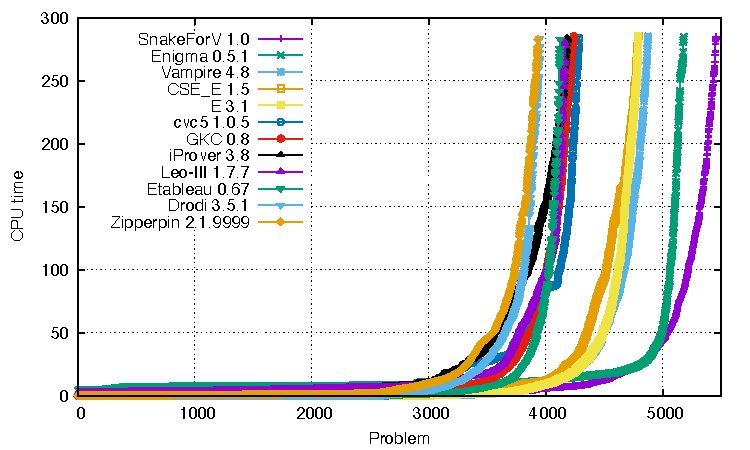
\includegraphics[width=0.75\textwidth]{Plots/FOF_THM_RFO_PPP/FOF_THM_RFO_PPP}
\vspace*{-1em}
\caption{CPU times for {\tt FOF\_THM\_RFO\_*}}
\label{PPPPlot}
\end{center}
\end{figure}

%--------------------------------------------------------------------------------------------------
\section{Analysis Process}
\label{Analysis}

Over time, decreasing difficult ratings of individual TPTP problems provide an indication of 
progress in the field \cite{SFS01}.
Individual problem ratings can be averaged over individual SPCs, or combinations of SPCs that
that describe compatible problem characteristics, to get an indication of progress for the SPCs.
Prior analysis, e.g., that in \cite{Sut17}, did just that.
Figure~\ref{OldRatingsPlot} is taken from \cite{Sut17}, where it was noted:
``The ratings generally show a downward trend - there has been progress!''.
It was also noted that:
``ratings can also increase when data from new systems is added to the TSTP.''
The counterintuitive increases in ratings as time progresses is caused by new systems becoming 
available.
A new system might not be subsumed, and the ratings of problems it solves go down. 
At the same time the new system might not be able to solve problems that the previously available
systems can, and the ratings of such problems go up.
For this work the analysis process has been refined to avoid this anomaly.

\begin{figure}[htb]
\begin{center}
\mbox{}
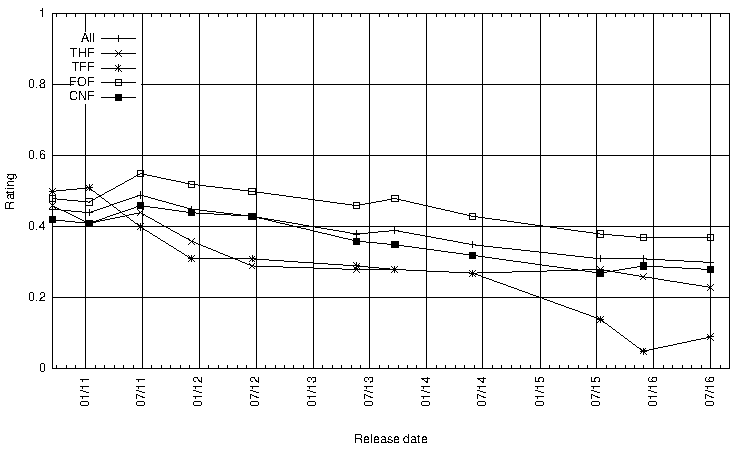
\includegraphics[width=0.75\textwidth]{Plots/RatingsDecline}
\vspace*{-1em}
\caption{Ratings decline from TPTP v5.0.0 to TPTP v6.4.0}
\label{OldRatingsPlot}
\end{center}
\end{figure}

Start from v6.2.0, released 14/07/15, by which time TSTP data was coming from StarExec, SPCs
were in place (but that doesn't matter because we care about only the current SPCs).

\begin{enumerate}
\item Extract all data from TSTP, starting from v6.2.0, per above.
\item Fill right for problems added after v6.2.0 if their rating started at 1.00. 
      This makes sense because if the a problem was unsolved when added, it would almost certainly 
      have been unsolved by earlier systems.
%      If the rating started below 1.00, that assumes that earlier systems would have been
%      equally able to solve it, which might be kind to those systems.
%      The result is less apparent progress before then.
\item Fill left for missing data
      \begin{itemize}
      \item Do not allowing a problem to become more difficult.
            That deals with new systems arriving and making a problem appear harder, but of course
            it does not.
      \item The new system makes some other problems become easier.
      \end{itemize}
\item Remove problems with missing ratings
\item Extract problems for a chosen set of SPCs 
      \begin{itemize}
      \item {\tt CNF\_UNS\_RFO\_NEQ\_*} $\cup$ {\tt CNF\_UNS\_RFO\_SEQ\_*} $\cup$ 
            {\tt CNF\_UNS\_RFO\_PEQ\_NUE} \\
            1115 + 2785 + 545 = 4445 problems in v8.2.0. NNNN in analysis.
      \item {\tt CNF\_UNS\_RFO\_PEQ\_UEQ} \\
            1140 problems. NNNN in analysis.
      \item {\tt CNF\_SAT\_RFO\_*} \\
            1044 problems. NNNN in analysis.
      \item {\tt CNF\_*\_EPR\_*} \\ 
            Decidable, so do {\tt SAT} and {\tt UNS} together.
            897 problems. NNNN in analysis.
      \item {\tt FOF\_THM\_RFO\_*} \\
            7204 problems. NNNN in analysis.
      \item {\tt FOF\_CSA\_RFO\_*} $\cup$ {\tt FOF\_SAT\_RFO\_*} \\
            707 + 322 = 1329 problems. NNNN in analysis.
      \item {\tt TF0\_THM\_*\_NAR} \\
            400 problems. NNNN in analysis.
      \item {\tt TF0\_THM\_*\_ARI} \\
            1176 problems. NNNN in analysis.
      \item {\tt TF0\_CSA\_*\_NAR} $\cup$ {\tt TF0\_SAT\_*\_NAR}. 
            35 + 120 = 155 problems. NNNN in analysis.
            Too few?
      \item {\tt TH0\_THM\_*\_NAR} \\
            3189 problems. NNNN in analysis.
      \end{itemize}
      Notes: TXF excluded because it started in only v8.0.0.
      Polymorphic TF1 and TH1 excluded because not enough systems are capable.
      Other excluded because too few problems.
\item Compute fraction of problems solved
\item Remove problems with ratings all 0.00 or all 1.00s -- they do no show any change
      in systems' performances because they are too easy or too hard.
\item Plot average rating by date.
      Zain needs to add date row.
\end{enumerate}

%--------------------------------------------------------------------------------------------------
\section{Evidence of Progress}
\label{Evidence}

Plots.
Commentary.

%--------------------------------------------------------------------------------------------------
\section{Conclusion}
\label{Conclusion}

This paper 

Ongoing and future work includes~\ldots

%--------------------------------------------------------------------------------------------------
\bibliographystyle{splncs04}
\bibliography{Bibliography}
%--------------------------------------------------------------------------------------------------
\end{document}
